%!TEX root = thesis.tex

\section{Reproducibility self-assessment}
\label{sec:reproducibility}

\begin{figure}[h]
  \centering
  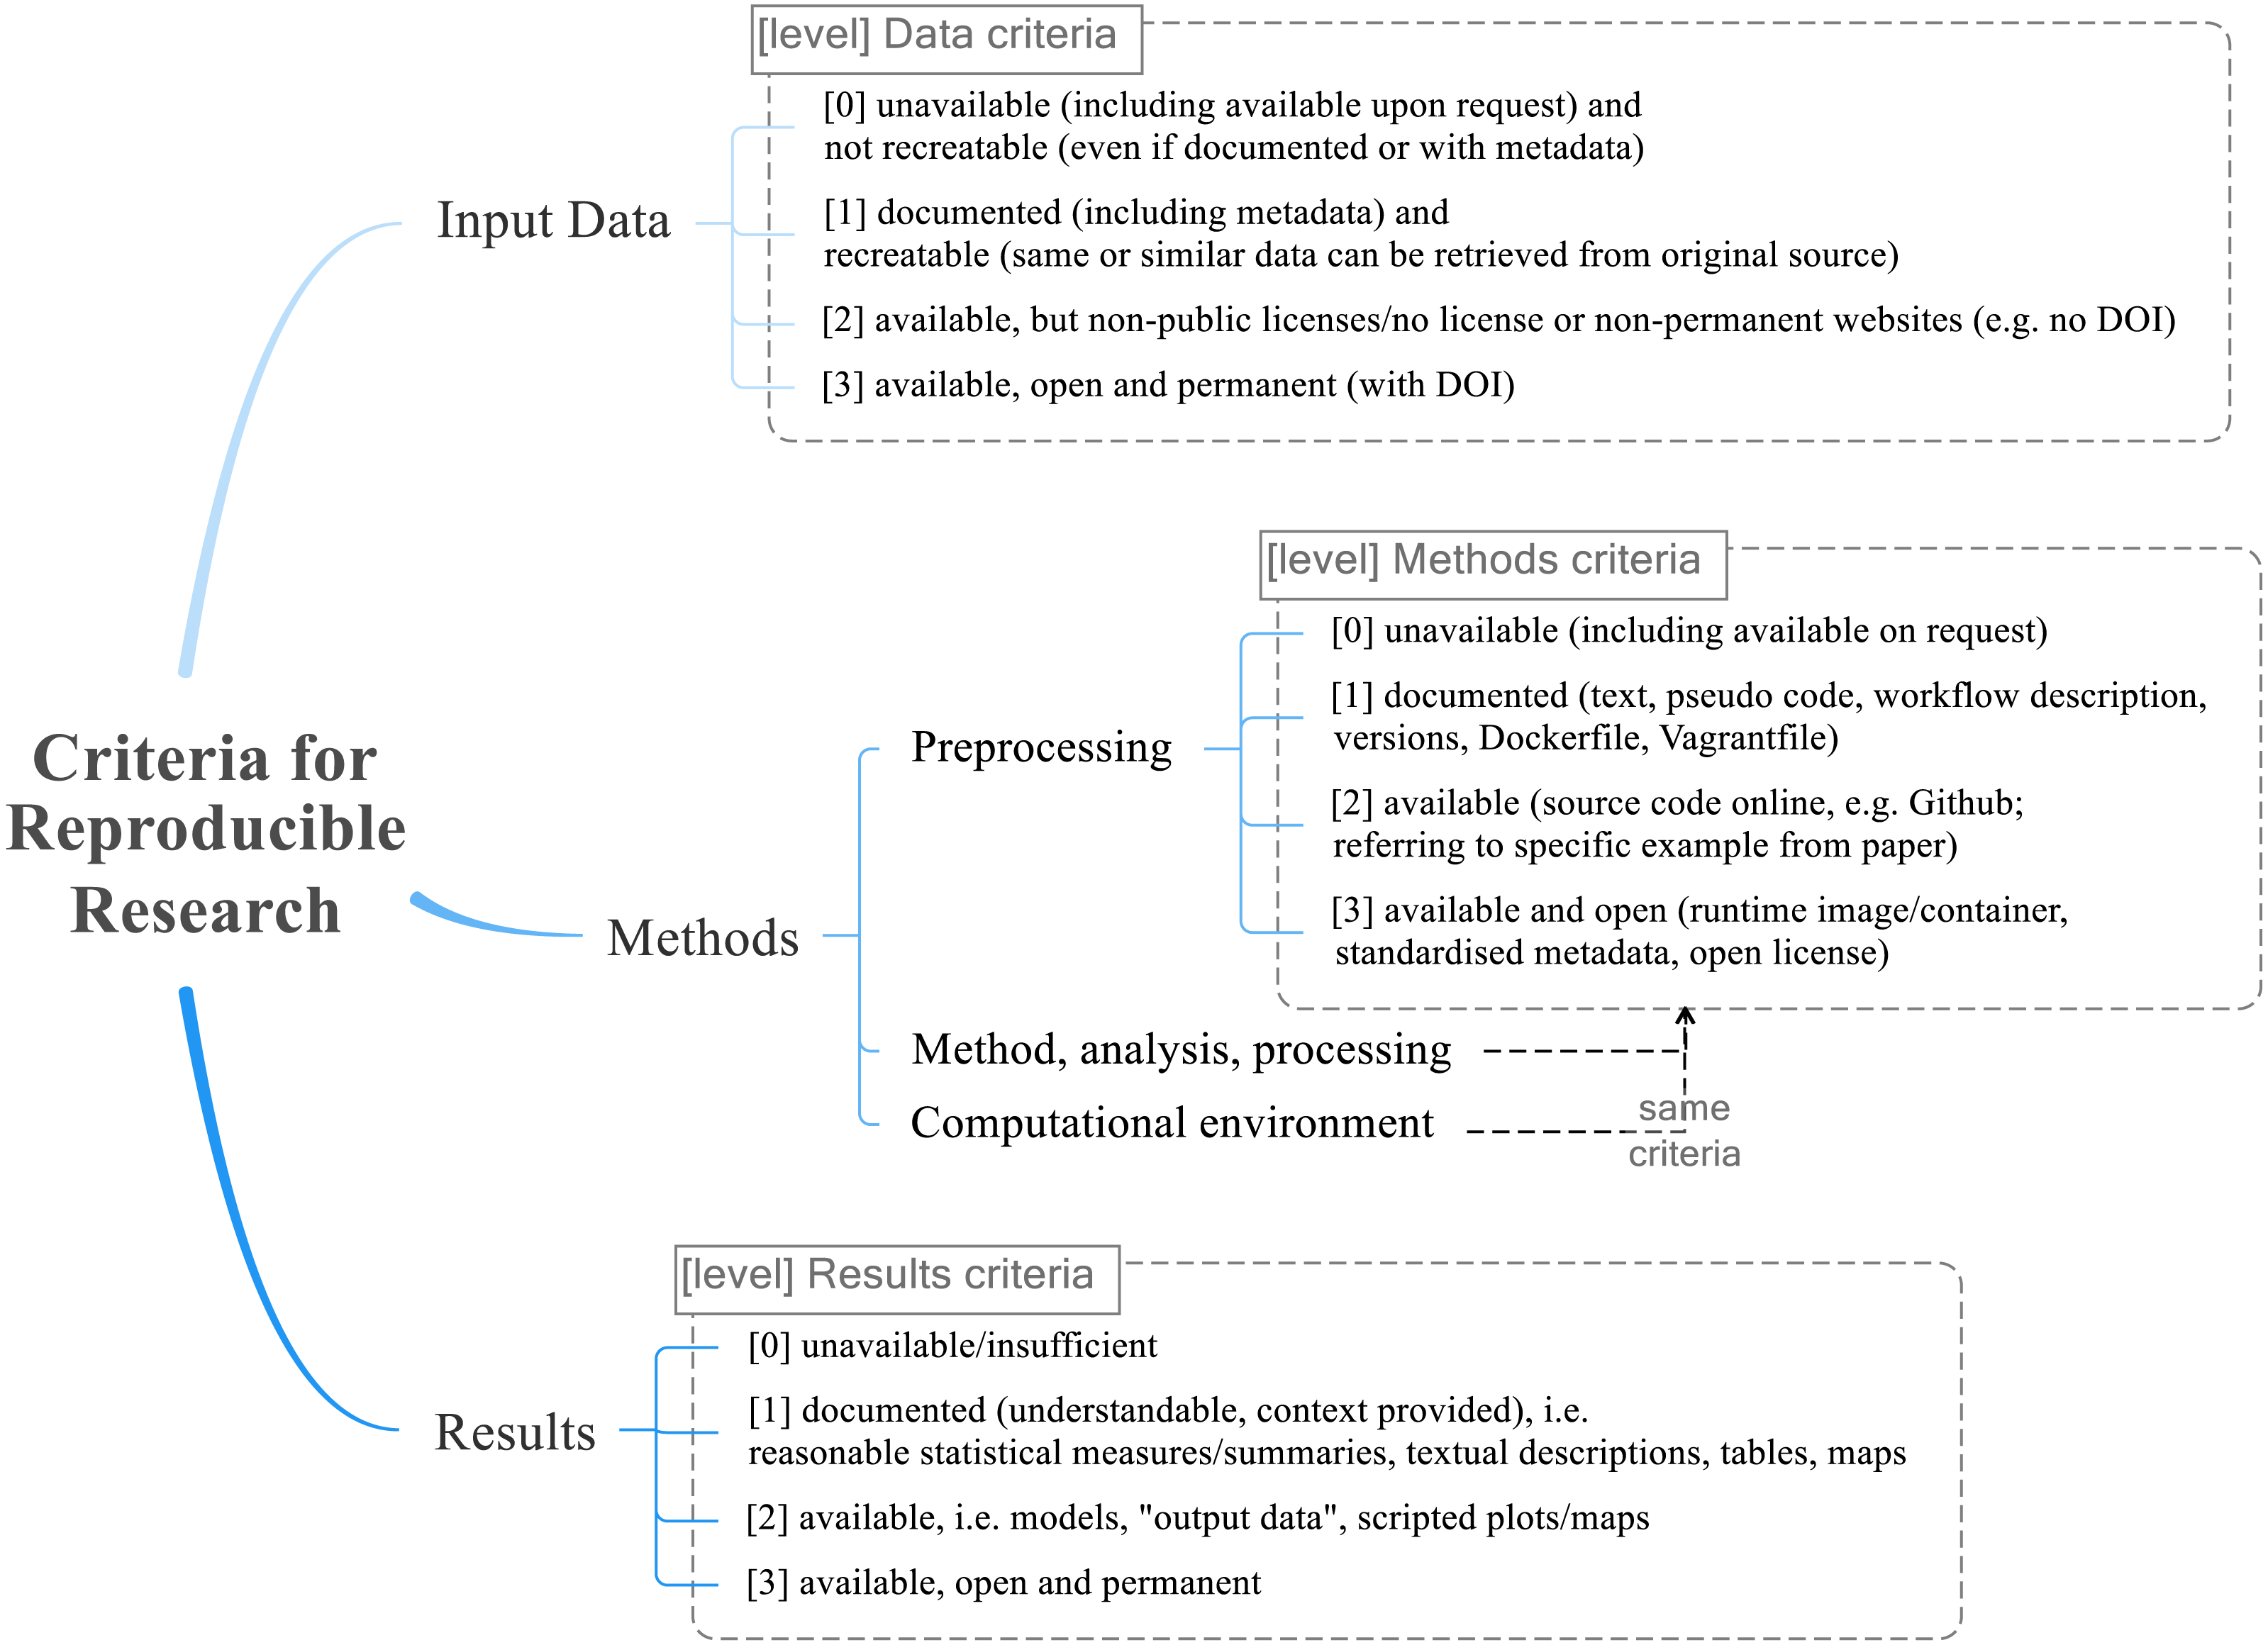
\includegraphics[width=0.9\linewidth]{figs/reproducibility_criteria.png}
  \caption{Reproducibility criteria to be assessed.}
\label{fig:reproducibility_criteria}
\end{figure}


Reproducibility self-assessment grades on the scale introduced in Figure \ref{fig:reproducibility_criteria}:

\begin{enumerate}
  \item Input data - \textbf{Grade = 2}
  \item Pre-processing - \textbf{Grade = 1}
  \item Methods - \textbf{Grade = 2}
  \item Computational environment - \textbf{Grade = 2}
  \item Results - \textbf{Grade = 2}
\end{enumerate}

\section{Self-reflection} 

It is both my personal belief and my faculty's standpoint that all parts of university research should be made public in a manner that allows all results to be reproduced, that are necessary to reach the research's conclusions. To exercise this notion in practice, I made 3 crucial logistical choices in consultation with my supervisors.

Firstly, all datasets used in my research are open data, accessible and reusable for both academic an commercial purposes. Secondly, my methods are not only well-documented, but the proof-of-concept implementation of my system design is available as an open-source Python application. Lastly, no tools were employed in the execution of the present research that require a commercial license. The only exception from this rule is FME, which I used to produce many of the visualisations shown here in the report. An academic license for FME can be obtained for free, although its use is not strictly necessary in terms of reproducing my results. There are other, equally suitable programs available that one can use to visualise my results.

To make it particularly easy for potential reusers to make use of my results, I maintain repositories hosting the source code of the present report, and that of the implementation. In addition, a package of example input datasets and output files (with various intermediate results included) are accessible via a link in the code repository. These are the same files on which most of the results described in the present report are based on. Reasonable efforts will be made to keep both the source repositories and the package of input/output files online at all times.

The only parts of my research whose reproducibility is somewhat less straightforward are the manual pre-processing and the commercial comparison steps. While the relevant steps have been described in-depth in this report, project files (e.g. for QGIS) and relevant source code are not available. These parts of the project can also be reproduced via basic knowledge of \ac{gis} tools and operations, and by following the steps outlined in this report. I decreased the pre-processing grade in the above list from 2 to 1 to reflect this limitation. Overall, the methods of the research still comply with the definition of grade 2, apart from the comparison with the commercial results.